\documentclass[12pt,a4paper]{article}
\usepackage{a4wide}

\usepackage{graphics} % for pdf, bitmapped graphics files
\usepackage{graphicx}
\usepackage{epsfig} % for postscript graphics
\usepackage{subfigure}
\usepackage{multirow}
\usepackage{float}
\usepackage{booktabs}
\usepackage{amssymb}
\usepackage{amsmath}
\usepackage{combelow}
\usepackage{hyperref}
\usepackage{natbib}
\renewcommand{\refname}{References}
%decrease space between captions and figures or tables
\usepackage[font=small,skip=0pt]{caption}

\renewcommand{\baselinestretch}{1.25}

\usepackage{textcomp,    % for \textlangle and \textrangle macros
            xspace}
\newcommand\la{\textlangle\xspace}  % set up short-form macros
\newcommand\ra{\textrangle\xspace}
\DeclareMathOperator*{\argmax}{argmax}

\graphicspath{{./Figs/}}
  
%\newcommand{\nr}[3]{\textlangle $#1 | \mathbf{#2} | #3$\textrangle}
\newcommand{\nr}[3]{$\langle#1 | \mathbf{#2} | #3\rangle$}

\title{\LARGE \bf
Determining Organizations and Their Sentiment in Full Length News Articles
}

\author{Keith Davis, Arturs Polis, Owain Steer}

\begin{document}

\maketitle



%%%%%%%%%%%%%%%%%%%%%%%%%%%%%%%%%%%%%%%%%%%%%%%%%%%%%%%%%%%%%%%%%%%%%%%%%%%%%%%%
%\begin{abstract} Batch effects are commonly present in biological data. This data must then be adjusted before further statistical analysis can take place. Many methods have been developed to remove batch effects. The paper ``Removal of batch effects using distribution-matching residual networks" Shaham et al. (2017) proposes a new approach to this problem that uses deep neural networks with residual connections to adjust data for batch effects\cite{Shaham2017}. We studied the method and repeated some of their experiments.
%\end{abstract}


%%%%%%%%%%%%%%%%%%%%%%%%%%%%%%%%%%%%%%%%%%%%%%%%%%%%%%%%%%%%%%%%%%%%%%%%%%%%%%%

\section{Problem Definition}
Given a collection of business news articles, we want to make it possible to automatically detect the sentiment expressed in regard of individual companies mentioned in the said articles. We aimed to explore how different ``deep learning" architectures can be used to accomplish this - namely to automatically extract the company/companies names in each news article as well as the sentiment per company. We wanted to see whether summarization of the article before the other steps would help in accuracy, given that per entity sentiment detection in longer article is generally challenging to the current aspect level sentiment models. \\ 

\begin{figure}[H]
  \centering
  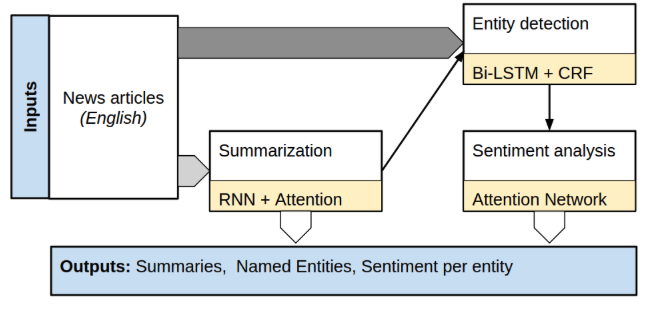
\includegraphics[scale=0.6]{approach.png}
  \caption{System Architecture}
  \label{fig:network_performance}
\end{figure}


\section{Our Approach}
There is an existing research on deep learning approaches to summarization, entity extraction and aspect based sentiment analysis within the larger domain of NLP. Therefore we decided to use already existing neural architecture implementations for each problem and pipeline the results of each step through to the next. 


As the work progressed, it became clear that different components rely on incompatible Python environments. We therefore used pickle archives and text files to pass inputs and outputs between the models, however with sufficient time and resource it would be possible to create a reasonably robust framework for running different components within the same environment. The source code for the project is available here: \\\mbox{\url{https://github.com/iamthevastidledhitchhiker/Zentropy}}

\section{Models}
\subsection{Summarization}
The Summarization component is based on the article by See et al\cite{See2017}. It uses a sequence-to-sequence model with attention mechanism, and consists of a Bi-directional LSTM encoder and LSTM decoder. Apart from attention, the model can copy out of vocabulary words from the source document using a pointer-generator mechanism. There is an optional coverage model that can be triggered at training time to take into account the parts of the source document that have already been covered to avoid having repetition in the generated summary. 

The TensorFlow implementation provided by the authors of the original paper did not allows import arbitrary test data easily, nor did it provide a mechanism to summarize one article at a time. There was also no way to easily export summaries for the use in other components in the pipeline. For these reasons the summarizer model code was forked and modified to enable the following: 1) Entering arbitrary articles for summarizations 2) Exporting summaries in a pickle format for use of other components in our pipeline. Version modified for this project is available here: \url{https://github.com/arpol/pointer-generator}. 

\subsubsection{Training and Results}

The model was trained on the CNN and Daily Mail summarization datasets: \\ \mbox{\url{https://cs.nyu.edu/~kcho/DMQA/}}, same as in the original paper, containing around 300k summarized news articles. For generating summaries we used 3 different models:
\begin{itemize}
\item \textbf{no coverage} - pre-trained model without coverage: \\(\mbox{\url{https://drive.google.com/file/d/0B7pQmm-OfDv7ZUhHZm9ZWEZidDg/view}})
\item \textbf{some coverage} - enabling the coverage and further training the pre-trained model for 2 days on a GPU 
\item \textbf{more coverage} - training the coverage enabled model for 2 more days 
\end{itemize}

Below is the example of output from the 3 models - as can be seen, more coverage does not necessarily provide better output: \hfill \break

\textbf{no coverage}

\begin{verbatim}
Tesla will be three times more powerful than any other battery system on earth.  
Musk says the system will be three times more powerful than  any other battery 
system on earth. Musk says the system will be three times more powerful than 
any other battery system on earth.
\end{verbatim}

\textbf{some coverage}
\begin{verbatim}
Tesla will partner with French renewable energy company Neoen to build the 
100-megawatt battery farm in South Australia. Tesla will partner with French
renewable energy company Neoen to build the 100-megawatt battery farm in 
South Australia.  Musk says the system  will be three times more powerful 
than any other battery system on earth.
\end{verbatim}

\textbf{more coverage}
\begin{verbatim}
Tesla will partner with French renewable energy company Neoen to build the 
100-megawatt battery farm in South Australia. the system will be three times 
more powerful than any other  battery system on earth. the system will be 
three times more powerful than any other battery system on earth.
\end{verbatim}

As can be seen, adding coverage may indeed remove blatant repetition, however, getting the full benefit of the coverage model would likely require a longer training period.

\subsection{Named Entity Recognition}
The model, based off of the model described in Lample et al\cite{Lample2016}, used a bidirectional LSTM with a CRF layer to tag named entities in IOBES format. As well as word embeddings this model also trained character based embeddings to capture prefix and suffixes of words being sensitive to capitalization of letters to help capture entities. The main 4 entities it tags being persons, organizations, locations and misc. We only used the organization tags when feeding to the aspect model.

We used a pre-trained english model, trained on CoNLL-2003. The training data consisted of 946 news articles which had 14,987 sentences, 203,621 tokens. With this training data the model has been recorded of having an F1 score of 90.94 on CoNLL-2003 test data.

The model was implemented in Theano using Python2.7 which caused several compatibility issues with the bulk of our project being in Python3. Instead we wrote to the input file (from the summarization model output) and manually ran a Python2.7 command via command line to bypass this. The output was also an arbitrary text file as shown in the example below. The output being too simple (rather than e.g a python dictionary or list) caused a decent amount of time being spent cleaning the data to be passed onto aspect based polarity.
\\ \\
\textbf{Input (NLTK Tokenized)}
\begin{verbatim}
Glencore PLC rode a wave of surging commodity prices in 2016 to return to a 
profit of $ 1.4 billion.
\end{verbatim}  \hspace{1cm} \\
\textbf{Output}

\begin{verbatim}
Glencore__B-ORG PLC__I-ORG rode__O a__O wave__O of__O surging__O 
commodity__O prices__O in__O 2016__O to__O return__O to__O a__O 
profit__O of__O $__O 1.4__O billion__O .__O
\end{verbatim}

\break

\subsection{Aspect-Level Sentiment Classification}
\subsubsection{Attention}
Initially, we used an implementation of the model described in Tang et al's paper\cite{Tang2016}, available here:  \url{https://github.com/ganeshjawahar/mem_absa}. However, getting the model to train properly even with 16gb of GPU memory proved exceptionally difficult. Rather than spend an inordinate amount of time debugging and reconfiguring the implementation, we switched to an implementation for Interactive Attention Networks as described by Ma et al\cite{Ma2017}. While this implementation was much faster to train and test, we ironically spent an inordinate amount of time debugging and reconfiguring the implementation to yield human-readable results. The author of the implementation seemed to care more about achieving good results for the SemEval competition rather than producing re-usable code that supports generalized text inputs. Data used was a modified version of the 19 000+ news article sentiment provided to the Deep Learning for NLP class. Data was structured into a plaintext file containing sentences with company names replaced with `aspect\_term`, the company name, and the sentiment polarity (positive, negative, and neutral).
\begin{verbatim}
The new agreement will cost aspect_term an estimated $1bn.
Volkswagen
negative
\end{verbatim}

Training the model for 300 epochs using 14629 training examples and validated on 3658 examples, achieving 68\% accuracy, however we were unable to test the model on data provided from the Named Entity Recognition outputs.

\subsubsection{Support Vector Machines}
After multiple failed attempts to test the attention-based model on the Named Entity Recognition outputs, a much simpler SVM approach was used instead. Using scikit-learn's svm.LinearSVC() and svm.LinearSVR() methods, we were able to construct classification and regression models to predict basic sentiment and offer somewhat passable aspect-level analysis. The models were trained using sentences with company names replaced with `aspect\_term` and labels corresponding to the original dataset polarity ([1.0, 0.0] for 100\% negative, [0.7, 0.3] for 70\% negative, and so on). Testing the trained models using a selected sentences of varying complexity, we found that model is fairly adept at recognizing sentiment for entire sentences, however it can become confused when presented with certain aspects or with different syntax. For example, the sentence \textit{aspect\_term won a lawsuit against Samsung} returns a predicted score of [0.7, 0.3] (negative for aspect\_term), however \textit{aspect\_term wins lawsuit against Samsung} returns a predicted score of [0.3, 0.7]. Building a more robust model through the use of word embeddings or POS-tagged sentences would likely improve the model. 

The SVR model was similarly tested, revealing that it cannot predict negative polarity, which is likely due to the fact that predicting a numerical polarity score is much more difficult than selecting between five classes. The model has been included for the sake of completeness.

\subsection{Results}
We ran tests on a 3986 testing set consisting of tuples  business news articles, salient organizations, and their corresponding polarity. We tested the simplified pipeline that performed summarizations and named entity recognition by simply counting how often one of the organizations detected by our NER matched the salient organization in the test set:

\begin{figure}[H]
  \centering
  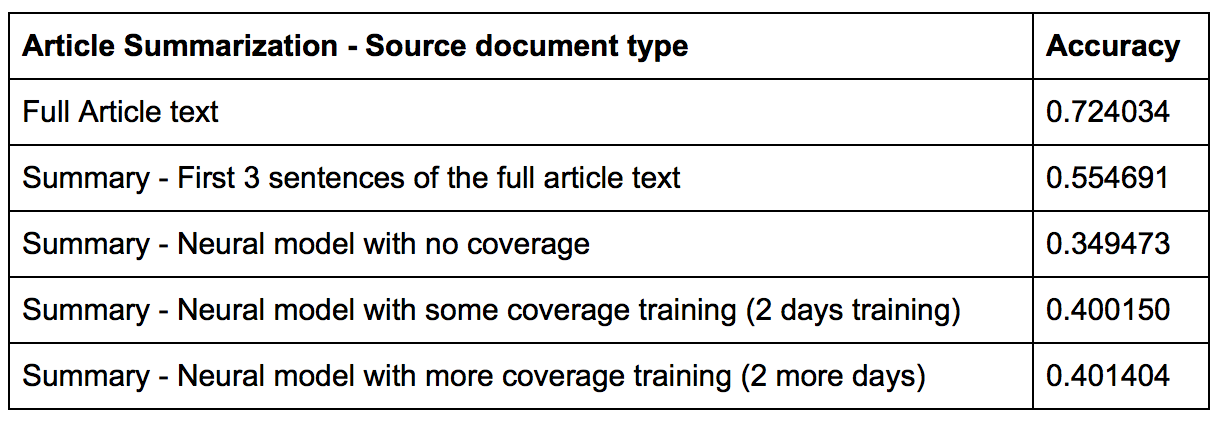
\includegraphics[scale=0.6]{results_summarization.png}
  \caption{Accuracy of salient named entity detection using 3986 business news articles}
  \label{fig:network_performance}
\end{figure}

The support vector classifier performed better with classifying the original article text and 3-sentence summaries, when comparing the predicted sentiment label with the original, human-classified sentiment label. Because the support vector classifier was trained using full article text, it is not surprising that it does not generalize as well on summaries. Additionally,  the classifier is heavily reliant on vocabulary and the summaries may not use the vocabulary necessary for the classifier to make reliable polarity predictions.
\begin{figure}[H]
  \centering
  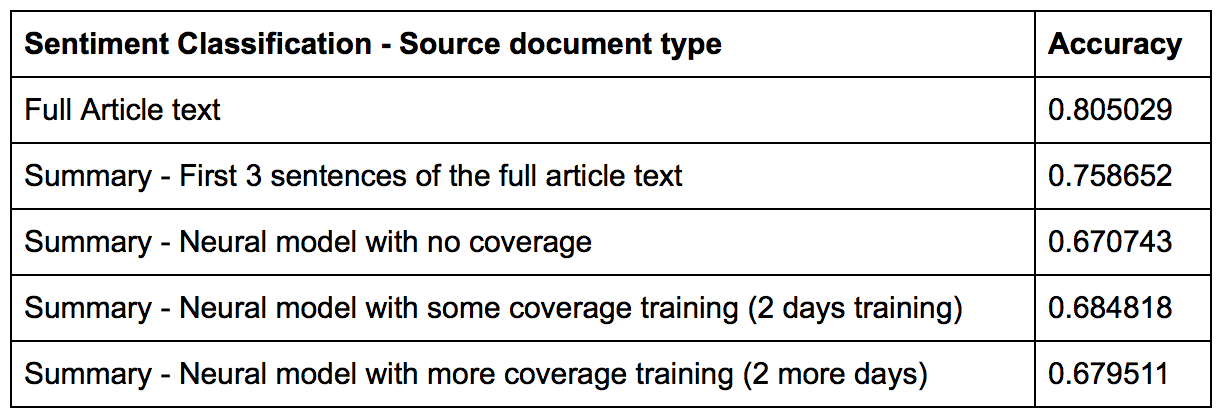
\includegraphics[scale=0.6]{results_sentiment.png}
  \caption{Accuracy of support vector classifier across input types}
  \label{fig:network_performance}
\end{figure}



\section{\label{Conclusions}Conclusions}
One issue lies in the fact the NER model is trained to find all named entities in the text, whereas for the data we used and intended applications, we only wanted the main organization(s) extracted from the text. Although the summarization hoped to mitigate this issue, performance would most likely been improved by only allowing a single entity output during training.

Given more time, patience, and knowledge of the inner workings of TensorFlow, it is likely that we could get the attention-based sentiment classification working properly, which would likely provide a more robust model. While the SVM-based classifier does not produce true aspect-level sentiment classification given the simplicity of its architecture, it performs well enough to function as a working prototype for the time being.

All in all, training each component individually means there is no end-to-end learning, and no way to communicate errors from one model to the next. If one module misses something, the whole chain is affected, and the error is unrecoverable by simple training. Furthermore, by testing the accuracy of the named entity recognition on different types of summaries as well as the full article, we saw consistent results with the current state of the art benchmarks of abstractive neural summarizers, where 3 sentence summaries are still the state of the art baseline.
\\ \\


\bibliographystyle{plain}
\bibliography{testbib}

%%%%%%%%%%%%%%%%%%%%%%%%%%%%%%%%%%%%%%%%%%%%%%%%%%%%%%%%%%%%%%%%%%%%%%%%%%%%%%%%

%%%%%%%%%%%%%%%%%%%%%%%%%%%%%%%%%%%%%%%%%%%%%%%%%%%%%%%%%%%%%%%%%%%%%%%%%%%%%%%

%%%%%%%%%%%%%%%%%%%%%%%%%%%%%%%%%%%%%%%%%%%%%%%%%%%%%%%%%%%%%%%%%%%%%%%%%%%%%%%%

%\bibliographystyle{IEEEtran}
%\bibliography{AsaReferences}

\end{document}

 
